\documentclass{article}

\usepackage[main=english,vietnamese]{babel}
\usepackage[T1]{fontenc}
\usepackage[utf8]{inputenc}
\usepackage[sexy]{evan}
\usepackage{matchsticks}
\usepackage{wrapfig}
\usepackage{listings}

\newtheorem{hint}{Hint}

\title{Solving Forty Two Problems by the Induction Principle - Part VI}
\author{Nghia Doan}
\date{\today}

\begin{document}

\maketitle

\begin{problem}[Problem Twenty Eight]
    Define a sequence $(a_n)$ by
    \[
        a_1 = 1, a_2 = 2, a_{n+2} = 2a_{n+1} - a_n + 2,\ \forall n\ge 1.
    \]

    Prove that $\forall m \ge 1,\ a_m a_{m+1}$ is also a term of this sequence.
\end{problem}

\begin{soln}
    First we prove by induction that 
    \begin{claim*}
        $a_n = (n-1)^2 + 1.$
    \end{claim*}
    \begin{subproof}
        It is easy to verify the base case. For the inductive step:
        \[
            2(n^2+1)-((n-1)^2+1) + 2 = n^2 + 2n + 2 = (n+1)^2+1.
        \]
    \end{subproof}

    Now, $\forall m \ge 1,$
    \[
        a_m a_{m+1} = ((m-1)^2 + 1)(m^2+1) = (m^2-2m+2)(m^2+1) = (m^2-m+1)^2+ 1 = a_{m^2-m+2}.
    \]
\end{soln}

\begin{problem}[Problem Twenty Nine]
    Let $a_1, a_2, \ldots$ be a sequence with 
    \[
        a_1 = 1,\ a_{n+1} = 
        \begin{cases}
            &a_n - 2 \text{\ if\ } a_n - 2 \not \in \{a_1, a_2, \ldots, a_n\} \text{\ and\ } a_n - 2 > 0,\\
            &a_n + 3 \text{\ otherwise}
        \end{cases}
    \]

    Prove that for every positive integer $k \ge 1,$ there exist $n$ such that 
    \[ 
        a_n = a_{n-1} + 3 = k^2.
    \]
\end{problem}

\begin{soln}
    It is easy to verify that by induction for a set of five numbers $5n+1, 5n+2, 5n+3, 5n+4, 5n+5,$
    \[
        a_{5n+1}=5n+1,\ a_{5n+2}=5n+4,\ a_{5n+3}=5n+2,\ a_{5n+4}=5n+4,\ a_{5n+5}=5n+3.
    \]

    The required statement follows.
\end{soln}

\begin{problem}[Problem Thirty]
    Let $x, y$ be real numbers such that the number $x+y,$ $x^2+y^2,$ $x^3+y^3,$ $x^4+y^4,$ are all integers.
    Prove that, for all $n \ge 5,$ $x^n + y^n$ is an integer.
\end{problem}

\begin{soln}
    First note that $2xy = (x+y)^2 - (x^2+y^2)$ so this is an integer.
    Furthermore
    \[
        2(x+y)^4 = 2(x^4+y^4) + 4(2xy)(x^2+y^2) + 3(2xy)^2 \Rightarrow 2 \mid 3(2xy)^2 \Rightarrow 2 \mid 2xy \Rightarrow xy \in \ZZ \quad (*)
    \]

    Now, with (*) and the identity
    \[
        x^{n+1} + y^{n+1} = (x+y)(x^{n} + y^{n}) - xy(x^{n-1} + y^{n-1})
    \]

    it is easy to prove by induction that $n \ge 5,$ $x^n + y^n.$
\end{soln}

\begin{problem}[Problem Thirty One]
    Let $a$ and $n$ be two positive integers such that $a^n - 1$ is divisible by $n.$
    Prove that the number $a+1, a^2 + 2, \ldots, a^n+n$ are all distinct modulo $n.$
\end{problem}

\begin{theorem*}[Euler's Theorem] 
    \label{theorem:euler-theorem}
    $a,n \in \ZZ,\ \gcd(a, n)=1 \Rightarrow a^{\varphi(n)}\equiv 1 \Mod {n},$
    where $\displaystyle \varphi(n) = n \prod_{p \mid n} \left(1 - \frac{1}{p} \right).$
\end{theorem*}

\begin{soln}
    We prove by induction. For $n=1$ the case case is clear with single term.
    Assume now that the statement is true for all integers less than $n \ge 2.$
    Let $k,$ the order of $a$ modulo $n,$ which is the least value such that $a^{k}\equiv 1 \Mod {n}.$
    
    From \nameref{theorem:euler-theorem}, $k < n,$ and from the condition given by the problem $n \mid a^n - 1,$
    we have $k \mid n.$ By induction hypothesis,
    \[
        a+1, a^2 + 2, \ldots, a^k+k
    \]

    are distinct modulo $k$. We prove now the statement:
    \[
        1 \le x \ne y \le n,\ a^x + x \not \equiv a^y +y \Mod{n}.
    \]

    Let $x = kz + t, y= ku+v,$ $(1\le t, uv\le k, 0 \le z, u < \frac{n}{k}.$ Then
    \[
        a^x \equiv a^t \Mod{n},\ a^y \equiv a^v \Mod{n}.
    \]
    
    \textit{Case 1:} $t \ne v,$ then 
    \[
        a^x + x \equiv a^t + t \not \equiv a^v + v \equiv a^y + y \Mod{n}.
    \]

    \textit{Case 2:} $t=v,$ then $z\ne u,$
    \[
        a^x +x \equiv a^t + kz + t = a^t + ku + v + k(z-u) \equiv a^y + y + k(z-u) \not \equiv a^y + y \Mod{n}.
    \]
\end{soln}

\begin{problem}[Problem Thirty Two]
    Let $n \ge 1,$ which is not divisible by 3. Show that
    \[
        x^3+y^3 = z^n
    \]
    has at least one solution $(x,y,z)$ where $x,y,z$ are positive integers.
\end{problem}

\begin{soln}
    The base case $n=1$ is obvious. For $n=2,$ we have $1^3 + 2^3 = 3^2.$
    
    Now, let assume that $(x_n,y_n,z_n)$ is a solution for the case $n,$ then
    \[
        (z_n)^{n+3} = (z_n^3)z_n^{n} = (z_n^3)(x_n^3+y_n^3) = (z_nx_n)^3 + (z_ny_n)^3
    \]

    Thus $(x_{n+3},y_{n+3},z_{n+3}) = (z_nx_n, z_ny_n, z_n)$ is a solution for $x^3+y^3 = z^{n+3}$ case.
\end{soln}

\begin{problem}[Problem Thirty Three]
    If $A_1, A_2, \ldots, A_n$ are any points in the plane, with any three not collinear,
    then there is a convex polygon $P$ such that some of $A_i$ are vertices of $P$ and the rest of the point are inside $P$.
    \textit{Note that $P$ is called the convex hull of $A_1, A_2, \ldots, A_n.$}
\end{problem}

\begin{center}
    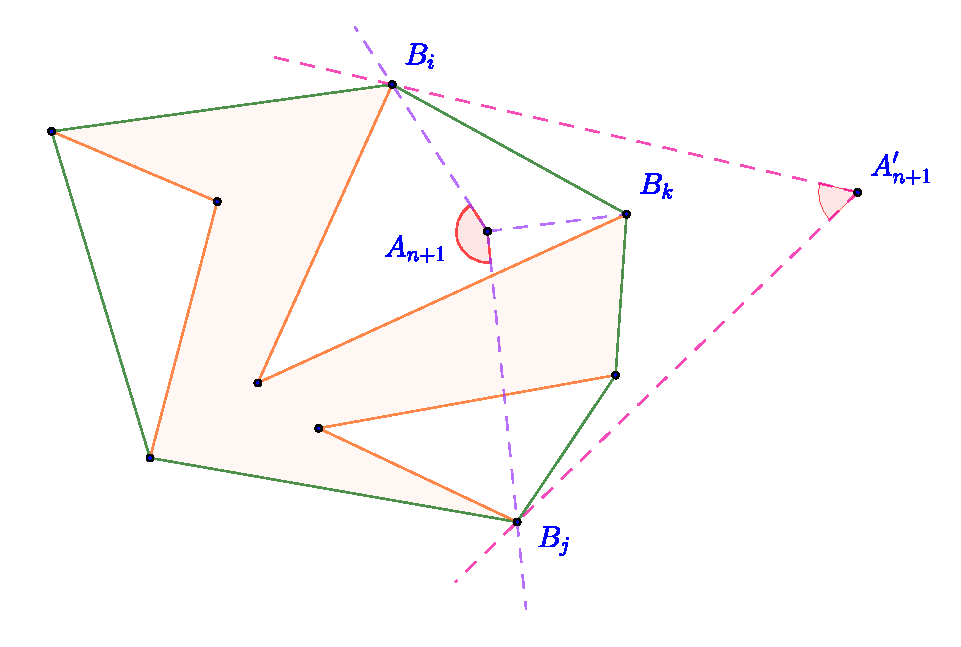
\includegraphics[width=10cm]{./svg/pdf/23-24-s5-o-p32.pdf}
\end{center}

\begin{soln}
    We prove by induction. The base case $n=3$ is trivial.

    Let's assume the hypothesis is true for $n.$ Now, Let $B_1 B_2 \ldots B_m$ ($m \le n$) be the convex hull of the polygon $A_1 A_2 \ldots A_n,$
    where $B_1, B_2, \ldots, B_m$ are some points of $A_1, A_2, \ldots, A_n.$
    
    Consider point $A_{n+1}.$ By the Extremal Principle there exists $B_i, B_j$ such that the measure of angle $\angle B_i A B_j$ (less than $180\dg$) is maximal.
    
    \textit{Case 1:} There exists point $B_k$ lies outside of this $\angle B_i A_{n+1} B_j.$
    $B_i, B_j, B_k$ cannot lie the same half-plane, otherwise one of $\angle B_i A_{n+1} B_k$ or $\angle B_k A B_j$ is larger than $\angle B_i A_{n+1} B_j,$
    which contradicting the choice of $\angle B_i A_{n+1} B_j.$ Thus $B_k$ like outside of the same half-plane formed by the angle $\angle B_i A_{n+1} B_j,$
    which means that $A_{n+1}$ is inside the triangle $\angle B_i B_k B_j,$ or inside the convex hull $B_1, B_2, \ldots, B_m.$
    Thus, $B_1, B_2, \ldots, B_m$ is the convex hull of $A_1 A_2 \ldots A_n A_{n+1}.$
    
    \textit{Case 2:} All $B_k$ other than $B_i, B_k$ lie inside of the $\angle B_i A'_{n+1} B_j.$
    Then, $B_1 B_2 B_i A_{n+1} B_j \ldots B_m$ is the convex hull of $A_1 A_2 \ldots A_n A_{n+1}.$
\end{soln}

\begin{problem}[Problem Thirty Four]
    $n$ is a positive integer, $n \ge 3.$

    (a) Prove that any $n-$gon (not necessarily convex) can be cut into triangles by non-intersecting diagonals.

    (b) Prove that the sum of the inner angles of any $n-$gon (not necessarily convex) is equal to $(n-2)180\dg$.
    Hence prove that the number of triangles into which an $n-$gon is cut by non-intersecting diagonals is $n-2.$
\end{problem}

\begin{center}
    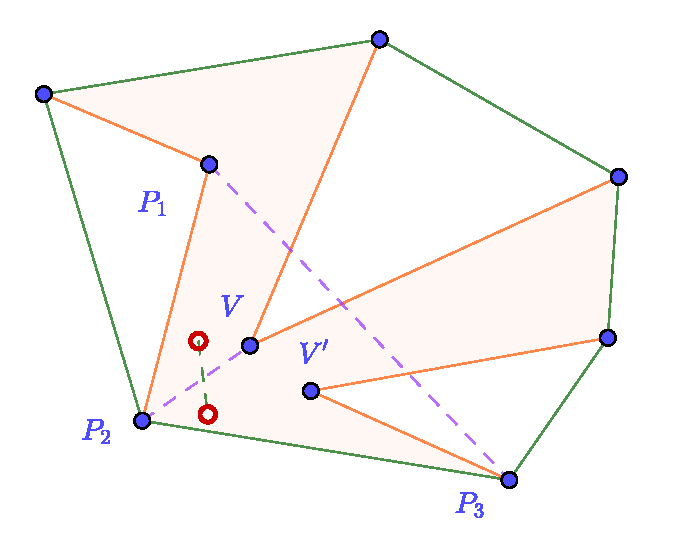
\includegraphics[width=6.5cm]{./svg/pdf/23-24-s5-o-p31.pdf}
\end{center}

\begin{soln}
    First, we use the Problem 33 for existence of a convex hull. Then
    \begin{claim*}
        Any $n-$gon $\cal{P}$ ($n \ge 4$) has at least one diagonal that completely lies inside it.
    \end{claim*}
    \begin{subproof}
        Let us index the vertices  $P_1P_2 \ldots P_n.$ Consider the convex hull $\cal{H}$. 
        $\cal{H}$ is a convex polygon, so it has a vertex, which will be one of the original vertices, WLOG, $A_2$.
        This ensures that the angle $P_1 P_2 P_3$ is less than $180\dg,$ i.e. if we take triangle $\triangle P_1 P_2 P_3$
        then part of the polygon $\cal{P}$ near $P_2$ is in the interior of $\cal{H}.$  
       
        Now if $P_1 P_3$ is an interior diagonal, then we are done.
        Otherwise, we know that there exists exterior part of the polygon inside $\triangle P_1 P_2 P_3.$
        In particular, there should be some vertices of $\cal{P}$ in there (see $V, V'$).
        Let $V$ be the vertex other than $P_2$ inside $\triangle P_1 P_2 P_3,$
        which is farthest away from the line $P_1 P_3,$.
        
        Then $VP_2$ lies in the interior of $\cal{P}$. Indeed, if there is a side of $\cal{P}$ that intersects $VP_2$,
        then one of the ends of is will be further away from $P_1 P_3$ than $V,$ but will still lie inside the triangle (see the points as hollow red circles)
        This would contradict the choice of $V.$
        Since the points inside the triangle near $P_2$ are in the interior of $\cal{P}$,
        then the whole segment is, which makes it an interior diagonal.
    \end{subproof}

    For the first question, we prove by induction. The base case of $n=3$ is clear.
    Now, for the inductive step, an interior diagonal divide it into two non-overlapping polygons, each with the number of sides less than $n.$
    By the hypothesis, both polygons can be cut into triangles by non-intersecting diagonals, thus the union set of triangles are the ones
    that the $n-$gon is cut into by non-intersecting diagonals.

    For the second question, the base case for the given hypothesis is clear.
    Now, for the inductive step, an interior diagonal divide it into two non-overlapping polygons, one with $k+1$ sides ($k$ of the $n-$gon plus the diagonal),
    the other with $n-k-1$ sides ($n-k$ sides from the $n-$gon plus the diagonals). 
    The sum of the inner angles of any $n-$gon now is equal to $(k-1) 180\dg + (n-k-1) 180\dg = (n-2)180\dg$.
    
    By the total measure of the sum of all angles, it implies that the number of such triangles is $n-2.$
\end{soln}

\begin{problem}[Problem Thirty Five]
    Point $O$ is inside (or on the boundary of) a convex $n-$gon $A_1 A_2 \ldots A_n.$
    Prove that among the angles $A_i O A_j$ ($1\le i \ne j \le n$) there are not fewer than $n-1$ non-acute ones.
\end{problem}

\begin{soln}
    We prove by induction based on $n$. For $n=3$ there is nothing to prove.

    Let consider $P_1P_2 \ldots P_n$ polygon, $n\ge 4.$ Let $p,q,r$ be such indexes that $O$ is inside $\triangle A_p A_q A_r.$
    Let $A_k \not \in \{ A_p, A_q, A_r \}.$
    By removing $A_k$ we receive a $(n-1)-$gon that we can apply the induction hypothesis to receive $n-2$ non-acute angles.
    Note that none of these triangles has $A_k$ as a vertex.

    Point $O$ now must be inside one of the triangles with vertices $A_k$ and two of $A_p, A_q, A_r.$
    WLOG let $O \in \triangle A_k A_q A_r.$ Then
    \[
        \angle A_k O A_q + \angle A_k O A_p = 360\dg - \angle Aq O A_r \ge 180 \dg.
    \]

    Hence, at least of of these two $\angle A_k O A_q, \angle A_k O A_p$ is a non-acute angles. Together with $n-2$ previously determined ones,
    they make $n-1$ non-acute angles.
\end{soln}

\end{document}